\section*{Le site}
\addcontentsline{ptc}{section}{Le site}
\label{sec:site}

Voici les différentes pages du site finalisé :

\begin{figure}[!h]
    \centering
    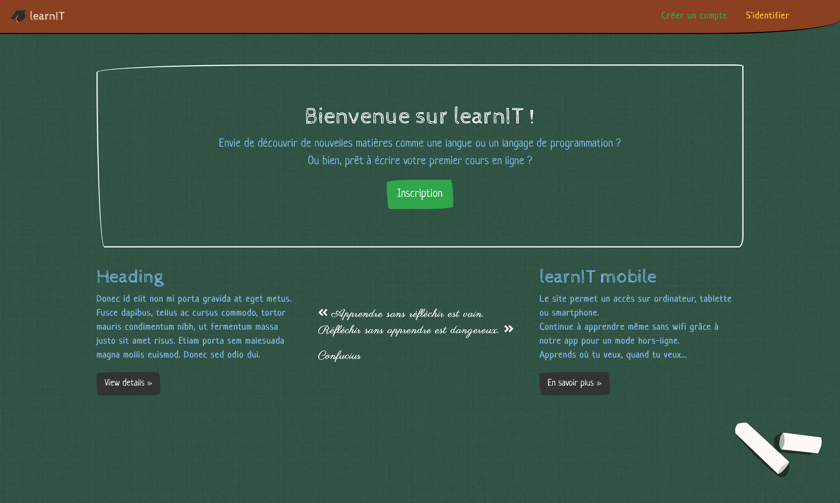
\includegraphics[scale=1]{textures/images/annexes/site/1a-Home.png}
    \caption{La page d'accueil}
\end{figure}
\begin{figure}[!h]
    \centering
    \includegraphics[scale=1]{textures/images/annexes/site/1b-CréerCompte.png}
    \caption{La page d'inscription}
\end{figure}

\newpage

\begin{figure}[!h]
    \centering
    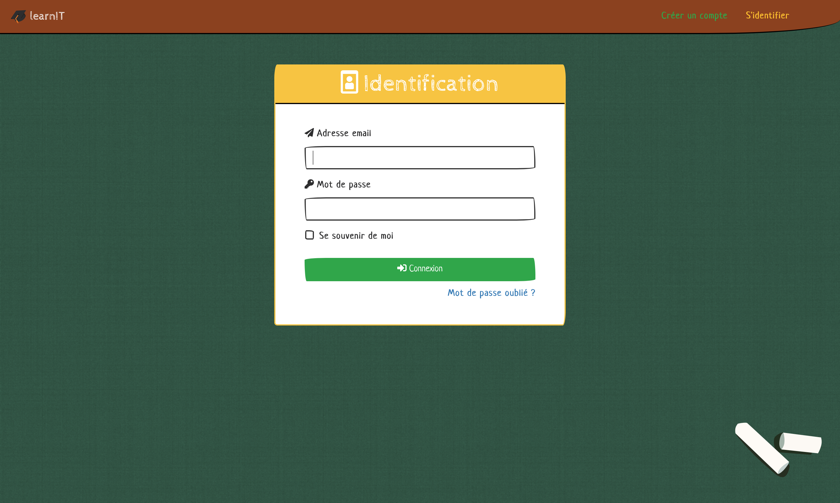
\includegraphics[scale=1]{textures/images/annexes/site/1c-Sidentifier.png}
    \caption{La page de connexion}
\end{figure}
\begin{figure}[!h]
    \centering
    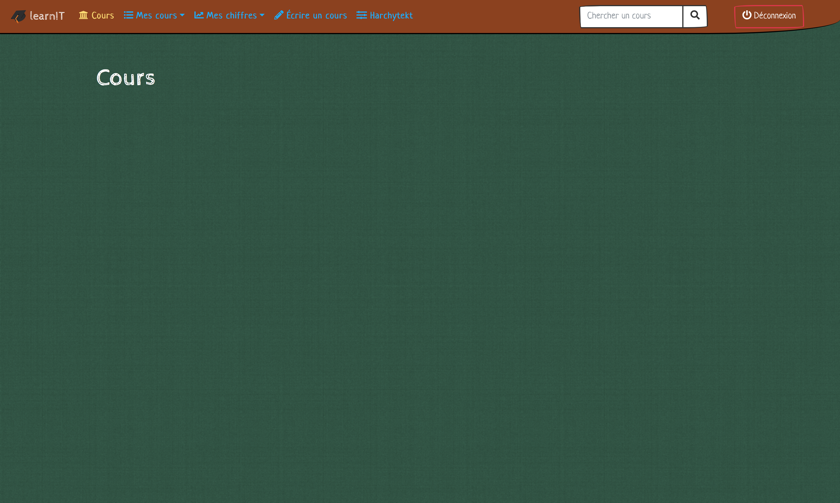
\includegraphics[scale=1]{textures/images/annexes/site/2-Cours.png}
    \caption{La liste des cours}
\end{figure}

\newpage

\begin{figure}[!h]
    \centering
    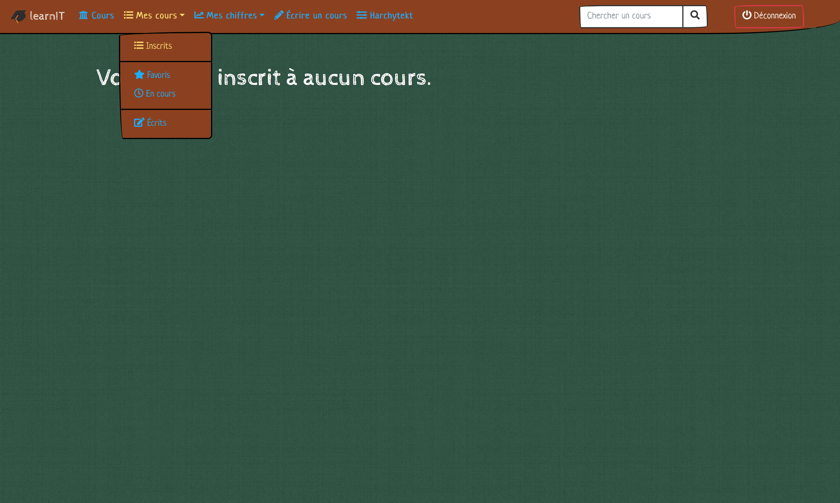
\includegraphics[scale=1]{textures/images/annexes/site/3-MesCours.png}
    \caption{La liste des cours auxquels l'utilisateur est inscrit}
\end{figure}
\begin{figure}[!h]
    \centering
    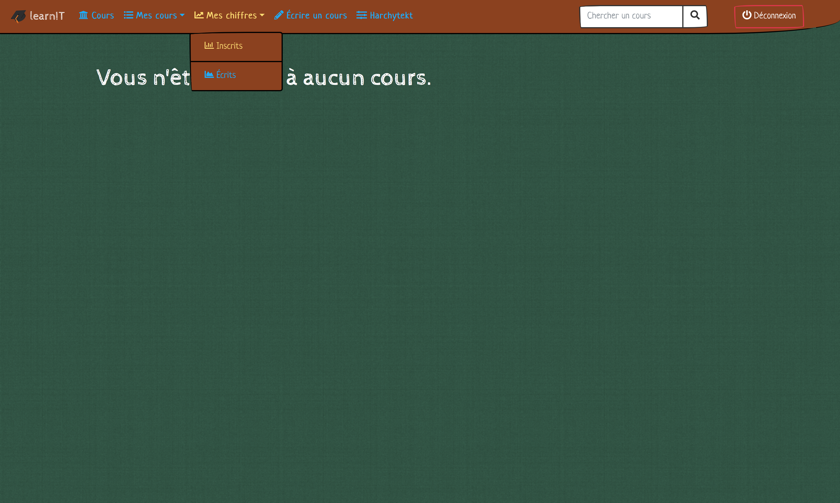
\includegraphics[scale=1]{textures/images/annexes/site/4-MesChiffres(Cours).png}
    \caption{La page des chiffres}
\end{figure}

\newpage

\begin{figure}[!h]
    \centering
    \includegraphics[scale=1]{textures/images/annexes/site/5-ÉcrireCours.png}
    \caption{La page de création d'un cours}
\end{figure}
\begin{figure}[!h]
    \centering
    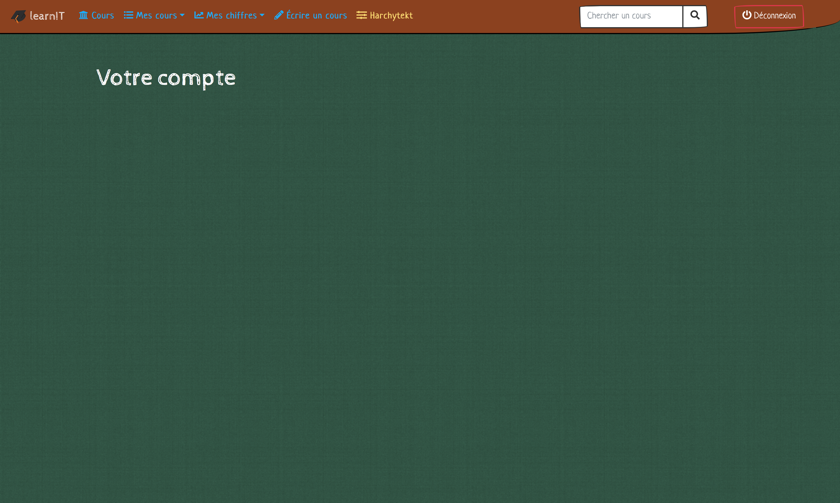
\includegraphics[scale=1]{textures/images/annexes/site/6-Compte(utilisateur).png}
    \caption{La page du compte utilisateur}
\end{figure}